\begin{questions}

\question{Consider the function $f(x)=\pi-x$, $0\leq x\leq \pi$.\newline

(a) Sketch the even, $2\pi$-periodic extension of $f$. Find the Fourier cosine series for $f$.
}
\begin{solution}
In the following figure we can see the even extension of $f$. 

\begin{figure}[H]
\centering     %%% not \center
{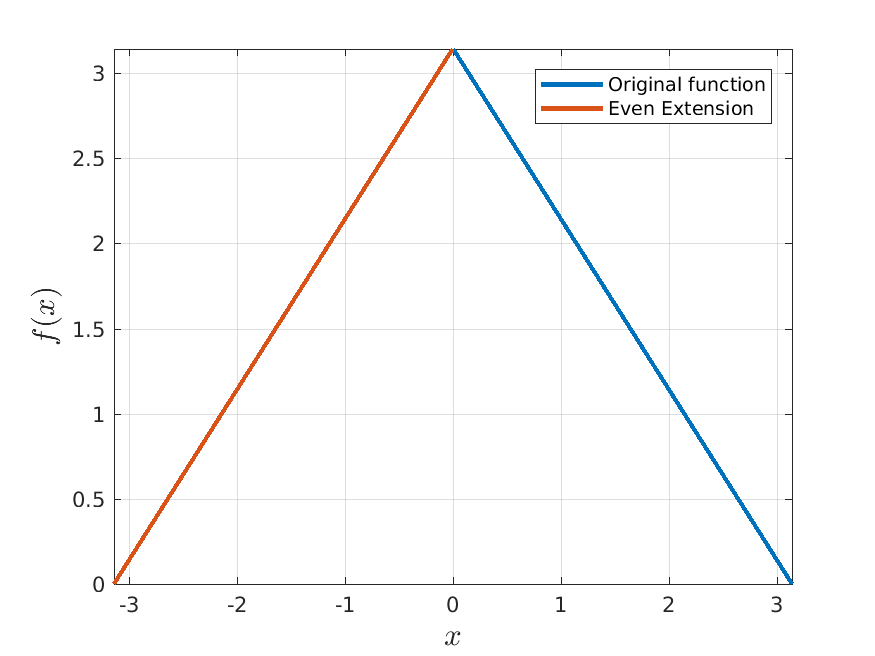
\includegraphics[scale=0.5]{evenExtension.png}}
\caption{Even extension of the function $f$.}
\end{figure}

Since the extended function is even, the Fourier series is going to be only a series of cosines. We now calculate the coefficients:
\begin{align*}
a_0=\frac{1}{2\pi}\int_{-\pi}^{\pi}f(t)dt=\frac{1}{\pi}\int_{0}^{\pi}(\pi-t)dt=\frac{1}{\pi}\left(\pi^2-\frac{1}{2} \pi^2\right)=\frac{\pi}{2},
\end{align*}
and
\begin{align*}
a_n=\frac{1}{\pi}\int_{-\pi}^{\pi}f(t)\cos(nt)dt&=\frac{2}{\pi}\int_{0}^{\pi}(\pi-t)\cos(nt)dt\\
&=\cancelto{0}{2\int_{0}^{\pi}\cos(nt)dt}-\frac{2}{\pi}\int_{0}^{\pi}t\cos(nt)dt\\
&=\frac{2}{n\pi}\int_{0}^{\pi}\sin(nt)dt\\
&=-\frac{2}{n^2\pi}\left.\cos(nt)\right]_0^{\pi},
\end{align*}
where we have used intergration by parts and that $\sin(n\pi)=\sin(0)=0$. Thus,
\begin{align*}
a_n=\frac{2}{n^2\pi}\left[1-\cos(n\pi)\right]= \left\{
\begin{array}{ll}
      0 & n $ even$ \\
      \frac{4}{n^2\pi} & n $ odd$ \\
\end{array} 
\right.
\end{align*}
Finally, the Fourier cosine series for $f$ is
\begin{align*}
FS(f)=\frac{\pi}{2}+\sum_{k=1}^{\infty}\frac{4}{\pi (2k+1)^2}\cos(kx)
\end{align*}
\end{solution}
\question{(b) Sketch the odd, $2\pi$-periodic extension of $f$. Find the Fourier sine series for $f$.
}
\begin{solution}
In the following figure we can see the odd extension of $f$. 

\begin{figure}[H]
\centering     %%% not \center
{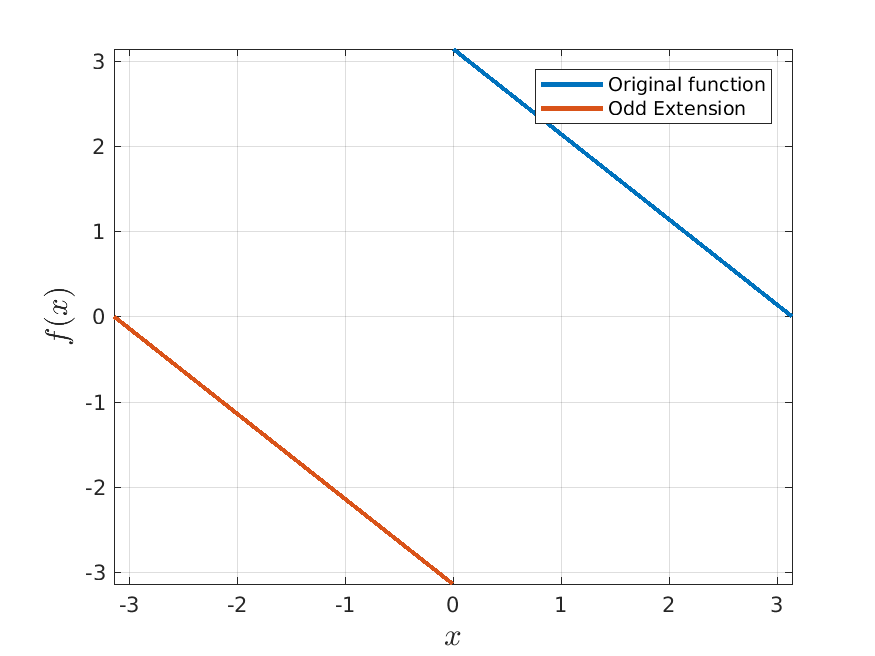
\includegraphics[scale=0.50]{oddExtension.png}}
\caption{Odd extension of the function $f$.}
\end{figure}

Since the extended function is odd, the Fourier series is going to be only a series of sines. We now calculate the coefficients:
\begin{align*}
b_n=\frac{1}{\pi}\int_{-\pi}^{\pi}f(t)\sin(nt)dt&=\frac{2}{\pi}\int_{0}^{\pi}(\pi-t)\sin(nt)dt\\
&=2\int_{0}^{\pi}\sin(nt)dt-\frac{2}{\pi}\int_{0}^{\pi}t\sin(nt)dt\\
&=-\frac{2}{n}\left.\cos(nt)\right]_0^{\pi}+\frac{2}{n\pi}\left.t\cos(nt)\right]_0^{\pi}-\cancelto{0}{\frac{2}{n\pi}\int_0^{\pi}\cos(nt)dt}\\
&=\frac{2}{n}\left[1-\cos(n\pi)\right]+\frac{2}{n\pi}\left[\pi\cos(n\pi)\right]\\
&=\frac{2}{n}
\end{align*}

Finally, the Fourier sine series for $f$ is
\begin{align*}
FS(f)=\sum_{n=1}^{\infty}\frac{2}{n}\sin(nx)
\end{align*}
\end{solution}
\question{(c) Sketch the $\pi$-periodic extension of $f$. Find the Fourier series for $f$.
}
\begin{solution}
In the following figure we can see the odd extension of $f$. 

\begin{figure}[H]
\centering     %%% not \center
{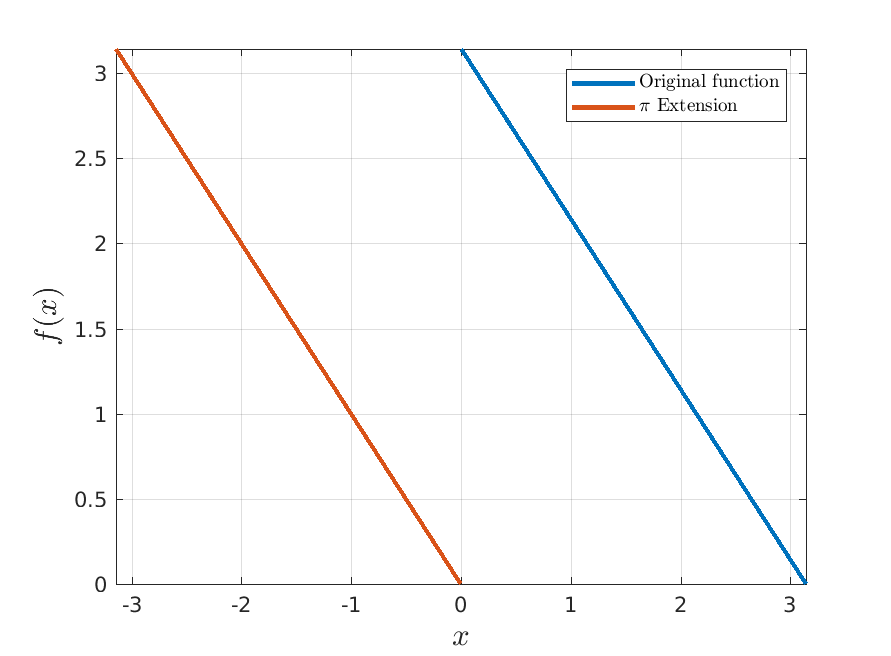
\includegraphics[scale=0.50]{piExtension.png}}
\caption{Extension of the function $f$.}\end{figure}

We first calculate the cosine coefficients starting with
\begin{align*}
a_0=\frac{1}{2\pi}\int_{-\pi}^{\pi}f(t)dt=\frac{1}{2\pi}\int_{-\pi}^{0}-tdt+\frac{1}{2\pi}\int_{0}^{\pi}(\pi-t)dt=\frac{\pi}{4}+\frac{\pi}{4}=\frac{\pi}{2}.
\end{align*}
For the rest of the cosine coefficients we note that we can apply the change of variables $y=-t$ the following way,
\begin{align*}
a_n=\frac{1}{\pi}\int_{-\pi}^{\pi}f(t)\cos(nt)dt&=\frac{1}{\pi}\int_{-\pi}^{0}-t\cos(nt)dt+\frac{1}{\pi}\int_{0}^{\pi}(\pi-t)\cos(nt)dt\\
&=\frac{1}{\pi}\int_{\pi}^{0}-(-y)\cos(-ny)(-dy)+\frac{1}{\pi}\int_{0}^{\pi}(\pi-t)\cos(nt)dt\\
&=-\frac{1}{\pi}\int_{\pi}^{0}y\cos(ny)dy+\int_{0}^{\pi}\cos(nt)dt-\frac{1}{\pi}\int_{0}^{\pi}t\cos(nt)dt\\
&=\frac{1}{\pi}\int_{0}^{\pi}y\cos(ny)dy+\int_{0}^{\pi}\cos(nt)dt-\frac{1}{\pi}\int_{0}^{\pi}t\cos(nt)dt\\
&=\int_{0}^{\pi}\cos(nt)dt\\
&=0
\end{align*}
where we have saved doing two of the integrals. Further, using the same change of variables,
\begin{align*}
b_n=\frac{1}{\pi}\int_{-\pi}^{\pi}f(t)\sin(nt)dt&=\frac{1}{\pi}\int_{-\pi}^{0}-t\sin(nt)dt+\frac{1}{\pi}\int_{0}^{\pi}(\pi-t)\sin(nt)dt\\
&=\frac{1}{\pi}\int_{\pi}^{0}-(-y)\sin(-ny)(-dy)+\frac{1}{\pi}\int_{0}^{\pi}(\pi-t)\sin(nt)dt\\
&=\frac{1}{\pi}\int_{\pi}^{0}y\sin(ny)dy+\int_{0}^{\pi}\sin(nt)dt-\frac{1}{\pi}\int_{0}^{\pi}t\sin(nt)dt\\
&=-\frac{1}{\pi}\int_{0}^{\pi}y\sin(ny)dy+\int_{0}^{\pi}\sin(nt)dt-\frac{1}{\pi}\int_{0}^{\pi}t\sin(nt)dt\\
&=-\frac{2}{\pi}\int_{0}^{\pi}y\sin(ny)dy+\int_{0}^{\pi}\cos(nt)dt\\
&=\frac{2}{n\pi}\left[y\cos(ny)\right]_0^{\pi}-\frac{2}{n\pi}\cancelto{0}{\int_0^{\pi}\cos(ny)dy}+\int_0^{\pi}\sin(nt)dt\\
&=\frac{2}{n}\cos(n\pi)-\frac{1}{n}\left(\cos(n\pi)-1\right)\\
&=\frac{1+\cos(n\pi)}{n} \left\{
\begin{array}{ll}
      \frac{2}{n} & n $ even$ \\
      0 & n $ odd$ \\
\end{array} 
\right.\\
\end{align*}
Finally, the Fourier series for $f$ is
\begin{align*}
FS(f)=\frac{\pi}{2}+\sum_{k=1}^{\infty}\frac{1}{k}\sin(kx)
\end{align*}
\end{solution}
\end{questions}
